\section{Scatterplot characterization}
\label{sec:visualizer:scatterplot}

\subsection{Characteristics of a ``good'' plot}
\label{sec:visualizer:scatterplot:goodplot}

The simplest scatter plot is one without any transformations on the data. This,
however, may not be the best way to ascertain independence for the user. This
notion is illustrated in Figure~\ref{fig:visualizer:cdf}. The left plot appears
to be independent as it's a cluster of points near the origin, but it's not
entirely clear due to the multitude of stray points outside of $y\in (-2,2)$ 
and $x\in(-1.5,1.5)$. By looking at the outliers, it could also be argued that 
there is some dependency. However, applying the CDF in both directions creates 
a plot distributed on (0,1). This transformation is non-destructive and 
preserves dependency in the data if it exists. The data is clearly independent 
as the points appear to be uniformly distributed within the box.

\begin{figure}[htb]
	\begin{center}
		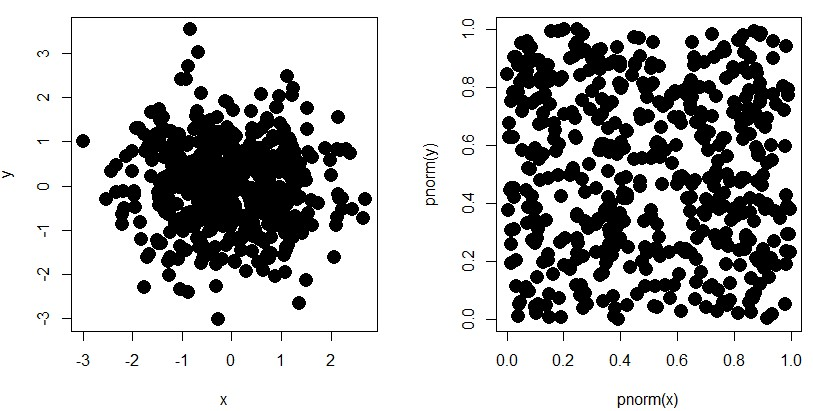
\includegraphics[width=0.75\linewidth]{ch-visualizer/figures/cdf}
		\caption[A plot of $y$ against $x$ after the CDF is applied in both
		directions.]{A plot of $y$ against $x$ with no transformation (left) 
		and after
			the CDF is applied in both directions (right). The code for this 
			example may be
			found in Appendix~\ref{sec:appendicies:cdf}}
		\label{fig:visualizer:cdf}
	\end{center}
\end{figure}

Restricting the scatter plot to a unit box allows analyst's visual systems to 
focus on locations where there is low spatial frequency, which is ideal for 
detecting dependence~\cite{hofert2016}. The effects of this concept can be 
progressively observed from left to right in 
Figure~\ref{fig:visualizer:hofertoldford} below.

\begin{figure}[htb]
	\begin{center}
		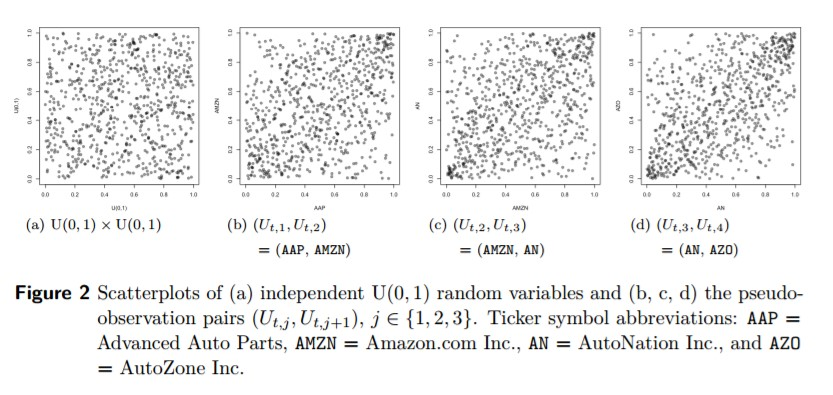
\includegraphics[width=1\linewidth]{ch-visualizer/figures/hofertoldford}
		\caption[Transformed scatter plots of independent $U(0,1)$ random 
		variables and pseudo-observation pairs $(U_{j},U_{j+1}),j\in 
		\{1,2,3\}$ which are more correlated the larger $j$ is.]{\textit{(a):} 
		Transformed scatter plots of independent $U(0,1)$ random variables. 
		\textit{(b,c,d):} Transformed scatter plots of the pseudo-observation 
		pairs $(U_{j},U_{j+1}),j\in \{1,2,3\}$. The variables are clearly more 
		correlated as $j$ increases; this trend can easily be observed due to 
		the nature of the unit box. Ticker abbreviations: 
		AAP = Advanced Auto Parts ($U_1$), AMZN = Amazon.com Inc. ($U_2$), 
		AN = AutoNation Inc. ($U_3$), AZO = AutoZone Inc. ($U_4$).
		Figure from Hofert and Oldford 2016 with slight 
		modifications~\cite{hofert2016}}
		\label{fig:visualizer:hofertoldford}
	\end{center}
\end{figure}

\subsection{Feature extraction from plot}
\label{sec:visualizer:scatterplot:features}

In order for the active learning classifier to properly understand and classify 
all $n \choose 2$ scatter plots in stage 1 and 2
(Sections~\ref{sec:visualizer:al} and~\ref{sec:visualizer:plotgeneration}), 
characteristic features must be extracted from each pairwise scatter plot. The 
more useful criteria there are, the more sophisticated the classification will 
be.

\subsubsection{Numerical features}

Our goal is to quantify various features of a scatter plot for the computer, 
and that does include numerical features. The following features are currently 
implemented in the VS: 

\tablespacing
\begin{itemize}
	\item \textbf{Correlation coefficients and their $p$-values:} Examples 
	include Pearson's, Spearman's, Kendall's, and distance correlation. See 
	Section~\ref{sec:intro:correlation} for more details on the various types 
	of coefficients.
	\item \textbf{Kullback-Leibler divergence criterion:} KL divergence 
	measures the difference between the probability distributions (which we 
	estimate to be Gaussian) of each pairwise set of variables. This feature is 
	non-symmetric, however, and reversing the order of the arguments 
	may yield a different result.
	\item \textbf{Chi-square test of independence and its $p$-value:} This 
	feature tests for independence among each pairwise set of variables 
	by comparing the frequency of categorical labels within each variable's 
	observations. As stock price data is not categorized by default, labels may 
	be generated given each observation's relative value (e.g. average, above 
	average, etc.). As with correlation, a low $p$-value indicates that 
	the two variables are dependent.
\end{itemize}
\bodyspacing 

\subsubsection{Visual features}

What is more challenging is to find a way to quantify the visual features of 
scatter plots. This may be done by looking for concentration of points in 
various spaces of the plot domain. The following features are currently 
implemented in the VS: 

\tablespacing
\begin{itemize}
	\item \textbf{Middle box criterion:} The percentage of points near the 
	center of the plot
	\item \textbf{LR criterion:} The percentage of points that lie above and 
	below the linear regression line
	\item \textbf{Clustering criterion:} The percentage quantile of the ratio 
	between the largest and next-largest distance
	\item \textbf{Visual trend criterion:} This is computed as 
	max(PosTrendCriterion, NegTrendCriterion). The positive trend criterion 
	(PosTrendCriterion) is computed from the percentage of points in the bottom 
	left and upper right while the negative trend criterion (NegTrendCriterion) 
	is computed from the percentage of points in the upper left and 
	bottom right. A higher visual trend criterion value suggests a greater 
	visual trend. 
\end{itemize}
\bodyspacing